% Lab 10 on Recursion
%
% CSE/IT 107: Introduction to Programming
% New Mexico Tech
%
\documentclass[11pt]{cselabheader}

%%%%%%%%%%%%%%%%%% SET TITLES %%%%%%%%%%%%%%%%%%%%%%%%%
\fancyhead[R]{Lab 10: Recursion}
\title{Lab 10: Recursion}

\begin{document}

\maketitle
\pagenumbering{roman}
\hrule

\begin{quote}
``A mirror mirroring a mirror.''

``In the end, we self-perceiving, self-inventing, locked-in mirages
are little miracles of self-reference.''
\end{quote}
\begin{flushright}
--- Douglas R. Hofstadter, I Am a Strange Loop
\end{flushright}

\hrule

\begin{figure}[H]
  \centering
  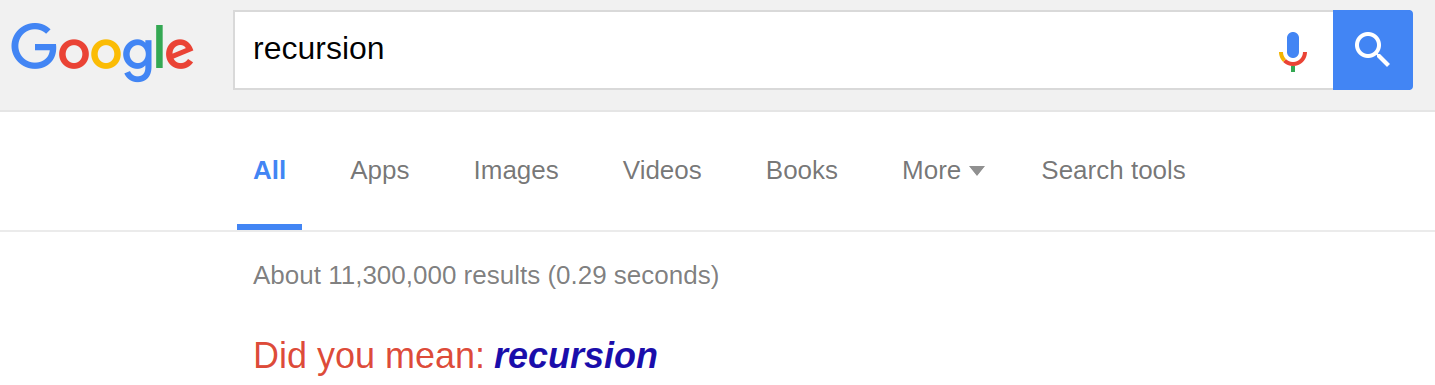
\includegraphics[width=\textwidth]{img/didyoumean.png}
  \caption{Google search for recursion (2016).}
\end{figure}

\begin{figure}[H]
  \centering
  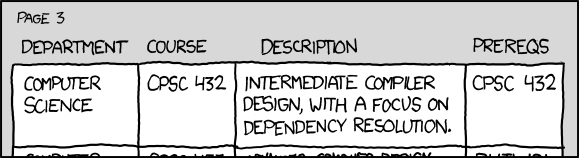
\includegraphics[width=0.5\textwidth]{img/xkcd_dependencies.png}
  \caption{Dependencies \url{http://xkcd.com/754/}}
\end{figure}

\hrule

\pagebreak
\section*{Introduction}
\addcontentsline{toc}{section}{Introduction}

You have learned about while loops, Python lists and how to manipulate
the elements in a list using for-loops and list comprehensions.  In
this lab you will learn about recursion.  Recursion can be used to
iterate through complicated data structures and to replicate the
functionality offered by while loops and for loops.  We will look at
some examples of recursive functions and the type of problems
recursion can help solve.

\tableofcontents

\pagebreak
\pagenumbering{arabic}

\section{A Function Can Call Itself}
\subsection{Functions}
One way to think about a function is to interpret calling a
function as copying and pasting the function body after setting the
parameters to specific values.

For example, the code on the left has several calls to two function
and can be translated into the code on the right. Notice the
body of each function is repeated multiple times.

\begin{multicols}{2}
\begin{python3code}
def greeting(recipient):
    return "Hello {}".format(recipient)

def greet_all_in_file(fname):
    with open(fname) as f:
        for line in f:
            print(greeting(line))

greet_all_in_file("names.txt")
greet_all_in_file(
    greeting("everyone") + ".txt")
\end{python3code}
\columnbreak
\begin{python3code}
# first call to greet_all_in_file
fname = "names.txt"
with open(fname) as f:
    for line in f:
        recipient = line
        print("Hello {}".format(
            recipient))

# second call to greet_all_in_file
recipient = "everyone"
fname = "Hello {}".format(recipient)
with open(fname) as f:
    for line in f:
        recipient = line
        print("Hello {}".format(
            recipient))
\end{python3code}
\end{multicols}

\subsection{A Short Recursive Function}

Can we do that same thing when we call this function?

\begin{python3code}
def count(n):
    print(n)
    count(n + 1)
count(0)
\end{python3code}

The answer is no. Although it is similar to this code:

\begin{python3code}
n = 0
print(n)
n = n + 1
print (n)
n = n + 1
print (n)
n = n + 1
print (n)
n = n + 1
print (n)
# this should continue forever
\end{python3code}

Note that this function never finishes.
It does the same thing as the following while loop.

\begin{python3code}
n = 0
while True:
    print(n)
    n += 1
\end{python3code}

The \pythoninline{count()} function is an example of a recursive call.
This means that within the function body the function calls itself
(see line 3). In this lab, we will explore similar functions.

\subsection{Termination}

How do you make a recursive function stop running?  Don't allow it to
call itself every time. For example, this function only calls itself
when its argument is big enough:

\begin{python3code}
def how_to_do_homework(problems):
    print("How to do {} homework problems".format(problems))
    if problems <= 1:
        print("Do the problem and then you're done.")
    else:
        problems -= 1
        print("Do the first problem and then do {} problems".format(problems))
        how_to_do_homework(problems)
\end{python3code}

Here is an example with \pythoninline{problems} set to 5.

\begin{verbatimcode}
How do you do 5 homework problems?
Do the first one and then do 4 problems.
How do you do 4 homework problems?
Do the first one and then do 3 problems.
How do you do 3 homework problems?
Do the first one and then do 2 problems.
How do you do 2 homework problems?
Do the first one and then do 1 problems.
How do you do 1 homework problems?
Do the problem and then you're done.
\end{verbatimcode}

\subsection{Examples with One Recursive Call}
\subsubsection{Traversing Data Structures}
Traversing a data structure means accessing every element stored within.
Here is an example function that adds 1 to every element in a list.
First, the function checks if the list is non-empty. If so, it adds
one to the first element and appends that element to the rest of
the list. The rest of the list is passed as an argument to the
recursive call.

\begin{python3code}
def add(elements):
    if len(elements) == 0:
        return []
    first_element = elements[0] + 1
    rest_of_list = elements[1:]
    return [first_element] + add(rest_of_list)
\end{python3code}

What happens when we call this function? Here is a step-by-step
example of running \pythoninline{add([1,2,3])}.

\begin{enumerate}
\item Input: \pythoninline{[1, 2, 3]}

First the function checks if the list is non-empty, then it adds 1 the
first element and calls itself with a shorter input.
\item Input: \pythoninline{[2, 3]}

This next function call also checks that the list is non-empty, it adds 1
to the first element and calls itself with an even shorter list.
\item Input: \pythoninline{[3]}

Same thing happens with this input.
\item Input: \pythoninline{[]}

There are no elements to add 1 to.
\item Output: \pythoninline{[]}

When this function receives the empty list, it returns an empty list.
\item Output: \pythoninline{[3 + 1] + []}

Function call 3 gets a value
\item Output: \pythoninline{[2 + 1] + [3 + 1] + []}

Function call 2 gets a value
\item Output: \pythoninline{[3 + 1] + [2 + 1] + [3 + 1] + []}

Finally, function call 1 gets the last two elements, appends the very
first element and then returns final result.
\end{enumerate}

When a function makes a recursive call by calling itself with a smaller input,
it is requesting that the same thing be done to that smaller input.
In this case, the first function call to \pythoninline{add} added 1 to the
first value of the list and then passed off the rest of the work to
function call 2. Function call 2 added 1 to the second element of the list,
and passed the rest of the work on to function call 3. This happened until
there were no more numbers in the list.

This code is an unrealistic way of traversing a list. It would be better to use
a list comprehension or a for-loop. Now let's look at an example where
recursion makes the problem much easier to solve.

%%% iterating through nested lists

\subsubsection{Creating Data}
Recursive calls are not just for iterating through data, they can also be used
to generate data.

factorial

\begin{python3code}

\end{python3code}

Long division, a common method of dividing a number by another number, can be
easily implemented using a recursive function. Here is how you divide a number
$a$ by another number $b$ to get the result $a / b$:
\begin{enumerate}
\item
\end{enumerate}

In code, this looks like

\begin{python3code}

\end{python3code}

draw spiral

\begin{python3code}

\end{python3code}

\begin{center}
% \includegraphics[width=\linewidth]{}
\end{center}

We can have multiple recursive calls in a function. To draw a type of tree,
we can use the turtle module to do the following.
\begin{enumerate}
\item If enough branches have been drawn, stop drawing.
\item Otherwise, draw a branch and draw two smaller trees at the top
of this branch.
\end{enumerate}

In code, this looks like:
\begin{python3code}
import turtle
def draw_tree(branch_size, maximum_branches):
    draw_tree(branch_size / 2, maximum_branches - 1)
    draw_tree(branch_size / 2, maximum_branches - 1)
draw_tree(100, 5)
\end{python3code}

This is a tree of height 5:
\begin{center}
% \includegraphics[width=\linewidth]{}
\end{center}

\subsection{Overview}
A typical recursive function calls itself one or more times.
It also has some sort of condition that causes it to stop calling itself.

Recursion is useful when dealing with nested data structures, such as
lists of lists. When a problem can be solved by solving smaller
versions of the problem, a recursive function might make a good
solution.  Recursion is used to sort lists of data, to read and run
computer programs, to solve mathematical problems, and for many other
problems.

\newpage
\section{Exercises}

\begin{ex}[palindrome.py] Write a recursive function that determines whether a
    string is a palindrome. A palindrome is a word that is the same forwards and
    backwards, for example ``abba''.

    The function should take in only one argument (the string to check) and
    return either \lstinline{True} or \lstinline{False}.

    It is required that your function must be recursive and take only one argument.
    This is not the easiest way to check if a string is a palindrome, but the goal
    is to solve a problem recursively, not to check if a value is a palindrome.
\end{ex}

\begin{ex}[list\_functions.py]
%%% add 1 to every sublist


%%% filter all sublists at depth N or more

Here is an example of using each function.
\begin{pyconcode}
>>> import list_functions
>>> list_functions.filter([], 1)
([], [[]])
>>> list_functions.filter([1,2,[3,4,[5,6]],[7]], 1)
([1,2], [[3,4,[5,6]], [7]])
\end{pyconcode}
\end{ex}

\begin{ex}[cesaro.py]
Use the Turtle module to draw the Cesaro torn line fractal.
This is the rule for drawing the fractal:
\begin{enumerate}
\item Draw a line from the starting position to the first midpoint.
\item Draw a Cesaro torn line fractal connecting the first midpoint to
the bottom midpoint.
\item Draw a Cesaro torn line fractal connecting the bottom midpoint
to the last midpoint.
\item Draw a line from the last midpoint to the final position.
\end{enumerate}

Here is a picture with the starting position, final position and the first,
bottom and last midpoints labeled:

\begin{center}
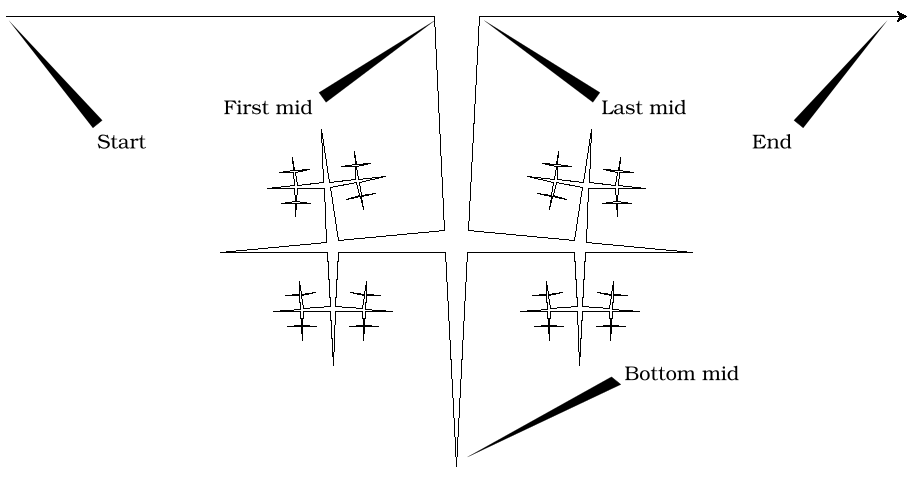
\includegraphics[width=\textwidth]{img/labeledcesaro.png}
\end{center}
\end{ex}

\section{Extra Credit Exercises}

\begin{extraex}[lsystem.py]
\end{extraex}

\begin{infobox}{Supplementary Files}
\end{infobox}

\newpage
\section{Submitting}

You should submit your code as a tarball. It should contain all files
used in the exercises for this lab. The submitted file should be named
\begin{center}
  \texttt{cse107\_firstname\_lastname\_lab10.tar.gz}
\end{center}

\begin{center}
  \textbf{Upload your tarball to Canvas.}
\end{center}

\listofexercises
\listofextraexercises

\end{document}
